\section{Control Charts}
\noindent\rule[\linienAbstand]{\linewidth}{\linienDickeDick}
The basis of a control chart is a statistical hypothesis test.

\subsection{Hypothesis test}
\noindent\rule[\linienAbstand]{\linewidth}{\linienDicke}

\textbf{Question:}\\
is $\left|\bar{x} - \mu_0\right|$ significant?\\
 - $\mu_0$ target value\\
 - $\bar{x}$ Arithmetic mean of the measurements


\textbf{Hypothesis:}\\
Two-sided statistical test to check the two alternative hypotheses:
\begin{equation}
  \begin{split}
    H_0:& \mu_0 = \bar{x} \text{ i.e. process is not disturbed}\\
    H_1:& \mu_0 \neq \bar{x} \text{ i.e. process is disturbed}
  \end{split}
\end{equation}

\paragraph{Statistical test:}\mbox{}\\
\textbf{Test statistic:} (z-test, since $\sigma$ is known)
\begin{equation}
  z = \frac{\bar{x}-\mu_0}{\sigma}\sqrt{n}
\end{equation}
\textbf{Critical value:} i.e. q-quantile of the normal distribution
\begin{equation}
  P(|z| \leq z_q) = q
\end{equation}
with $q = 1- \frac{\alpha}{2}$, where $\alpha = 0.0027 \rightarrow z_q \approx 3$\\

\textbf{Statistical conclusion:}\\
If $\leq |z| \ z_q \rightarrow$ accept null hypothesis, i.e. process is not disturbed.\\
If $< |z| \ z_q \rightarrow$ reject null hypothesis, i.e. process is disturbed.\\

Reverse it and determine acceptance and rejection limits of the test!

\textbf{Control limits:}
\begin{equation}
  UCL = \mu_0 + z_q \frac{\sigma}{\sqrt{n}} \;\;\;\;\; LCL = \mu_0 - z_q \frac{\sigma}{\sqrt{n}}
\end{equation}

\textbf{Statistical conclusion:}\\
If $LCL \leq \bar{x} \leq UCL \rightarrow$ process is not disturbed.\\
If $\bar{x} < LCL or UCL < \bar{x} \rightarrow$ process is disturbed.\\

Problem: In general, process standard deviation is unknown.\\
 - Monitoring the mean and the variation of a process.\\
 - First, monitoring the variation, then (if variation under control) monitoring the mean.\\

Solution: Control charts! :)




\subsection{The Control Chart}
\noindent\rule[\linienAbstand]{\linewidth}{\linienDicke}
\begin{figure}[H]
  \centering
  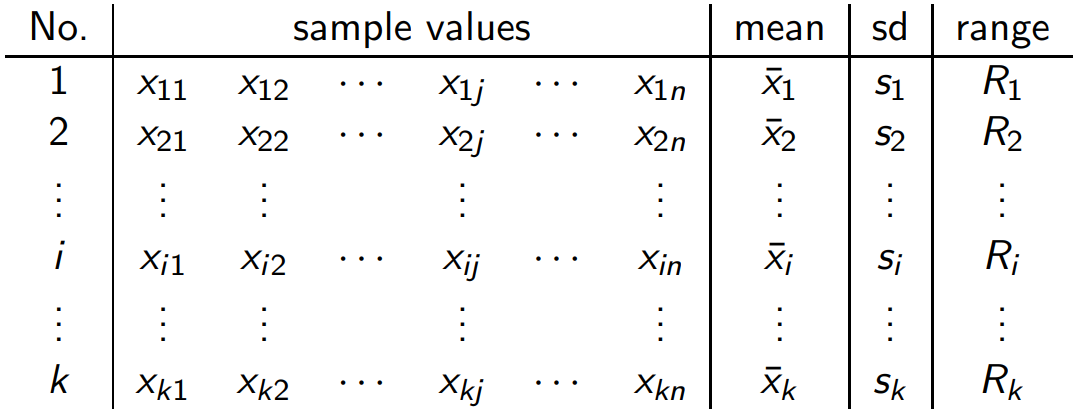
\includegraphics[width = 0.8\linewidth]{Pics/2.1.png}
  \caption{Data Set with Mean, Standard Deviation and Range}
  \label{2.1}
\end{figure}

\textbf{Mean values}
\begin{equation}
  \bar{x}_i = \frac{1}{n} \sum_{j=1}^n x_{ij}
\end{equation}

\textbf{Standard deviations}
\begin{equation}
  s_i = \sqrt{\frac{1}{n-1} \sum_{j=1}^n \left(x_{ij} - \bar{x}_i\right)^2}
\end{equation}

\textbf{Ranges}
\begin{equation}
  R_i = max\left \{x_{ij} | j \in \left \{1,...,n\right \} \right \} - min\left \{x_{ij} | j \in \left \{1,...,n\right \} \right \}
\end{equation}
for all $i \in \left \{1,...,k\right \}$

\subsection{Control Chart for $\bar{x}$ and R}
\noindent\rule[\linienAbstand]{\linewidth}{\linienDicke}
\paragraph{R Chart}\mbox{}
\textbf{Centerline}
\begin{equation}
  \bar{R} = \frac{1}{k} \sum^k_{i=1} R_i
\end{equation}

\textbf{Control limits}
\begin{equation}
    UCL = D_4 \bar{R}; \;\;\;\;\; LCL = D_3 \bar{R}
\end{equation}

\paragraph{$\bar{x}$ Chart based on R chart}\mbox{}\\
\textbf{Control limits}
\begin{equation}
  \begin{split}
    UCL = \mu + 3 \frac{\sigma}{\sqrt{n}}; \;\;\;\;\; LCL = \mu - 3 \frac{\sigma}{\sqrt{n}}
  \end{split}
\end{equation}
Problem: $\mu$ and $\sigma$ are in general unknown and must be estimated from the process data.\\
Two-stage process:\\
 - Make sure that the process standard deviation (R chart) is under statistical control. That is, if some samples are out of bounds, it is recommended
to omit these measurements and recalculate the limits.\\
 - Use $\bar{R}$ to estimate the process standard deviation.\\

\textbf{Centerline}\\
We know that for an independent sample $x_1, ... ,x_n$ from a normal distribution with parameters $\mu$ and $\sigma$ the mean
\begin{equation}
  \bar{x} = \frac{1}{n} \sum_{j=1}^n x_{j}
\end{equation}
satisfies
\begin{equation}
  E\left(\bar{x}\right) = \mu \;\;\;\; and \;\;\;\; Var\left(\bar{x}\right) = \frac{\sigma^2}{n}
\end{equation}

The mean is an unbiased estimator with the standard error
\begin{equation}
  SE\left(\bar{x}\right) = \frac{\sigma}{\sqrt{n}}
\end{equation}

Assumption: R chart is under statistical control.\\
 - The value $\bar{R}$ is a reliable estimate for the mean range.\\
 - The value $\bar{R}$ is a reliable estimate for the process standard deviation
\begin{equation}
  \hat{\sigma} = \frac{\bar{R}}{d_2}
\end{equation}

Any samples excluded for construction of the R chart should also be disregarded for construction of the $\bar{x}$ chart.
This results in a sample of $k^\star$ valid samples, (where $k^\star$ denotes the reduced number of samples).
Mean values of $\bar{x}_1, ... ,\bar{x}_{k^\star}$ provide an estimate of $\mu$, i.e
\begin{equation}
  \bar{\bar{x}} = \frac{1}{k^\star} \sum^{k^\star}_{i=1} \bar{x_i}
\end{equation}

\textbf{Control limits}
\begin{equation}
  \begin{split}
    UCL =& \bar{\bar{x}} + 3\frac{\bar{R}}{d_2} \frac{1}{\sqrt{n}}\approx \bar{\bar{x}} + A_2 \bar{R}\\
    UCL =& \bar{\bar{x}} - 3\frac{\bar{R}}{d_2} \frac{1}{\sqrt{n}}\approx \bar{\bar{x}} - A_2 \bar{R}
  \end{split}
\end{equation}

\subsection{Control Chart with $\bar{x}$ and s}
\noindent\rule[\linienAbstand]{\linewidth}{\linienDicke}

\paragraph{s Chart}\mbox{}\\
\textbf{Centerline}
The centreline of the s chart is denoted by $\bar{s}$ and is calculated from the arithmetic mean of the standard deviations\\
\begin{equation}
  \bar{s} = \frac{1}{k} \sum^k_{i=1} s_i
\end{equation}

\textbf{Control limits}
\begin{equation}
    UCL = B_4 \bar{s}; \;\;\;\;\; LCL = B_3 \bar{s}
\end{equation}

\paragraph{$\bar{x}$ Chart based on s chart}\mbox{}\\
Using an s chart of a process that is under control, the process standard deviation can be estimated by
\begin{equation}
  \hat{\sigma} = \frac{\bar{s}}{c_4}
\end{equation}
Any samples excluded for construction of the s chart should also be disregarded for construction of the $\bar{x}$ chart.
This results in a sample of $k^\star$ valid samples, (where $k^\star$ denotes the reduced number of samples).
Mean values of $\bar{x}_1, ... ,\bar{x}_{k^\star}$ provide an estimate of $\mu$, i.e
\begin{equation}
  \hat{\mu} = \bar{\bar{x}} = \frac{1}{k^\star} \sum^{k^\star}_{i=1} \bar{x_i}
\end{equation}

\textbf{Control limits}
\begin{equation}
  \begin{split}
    UCL =& \bar{\bar{x}} + 3\frac{\bar{s}}{c_4} \frac{1}{\sqrt{n}} \approx \bar{\bar{x}} + A_3 \bar{s}\\
    UCL =& \bar{\bar{x}} - 3\frac{\bar{s}}{c_4} \frac{1}{\sqrt{n}} \approx \bar{\bar{x}} - A_3 \bar{s}
  \end{split}
\end{equation}

\subsection{Individual Control Charts}
\noindent\rule[\linienAbstand]{\linewidth}{\linienDicke}
Individual control charts have exactly one measurement per sample.\\
Problem: You cannot estimate variability from a single measurement.
Idea: Use variation of two adjacent measurements.\\

\textbf{Moving ranges}
\begin{equation}
  MR_i = |x_{i+1} - x_i|
\end{equation}
for all $i \in \left\{1,...,n-1\right\}$.\\

\textbf{Arithmetic mean of the moving ranges}
\begin{equation}
  \overline{MR} = \frac{1}{n-1} \sum_{i=1}^{n-1}MR_i
\end{equation}
\textbf{Estimated process standard deviation}
\begin{equation}
  \hat{\sigma} = \frac{\overline{MR}}{d_2} = \frac{\overline{MR}}{1.128}
\end{equation}
Since two neighboring measurements were used to calculate the moving ranges we have $d_2 = 1.128$.\\

\textbf{Centerline}\\
The centerline for the individuals control chart is the arithmetic mean of the measured values.
\begin{equation}
  \bar{x} = \frac{1}{k} \sum^k_{i=1} x_i
\end{equation}

\textbf{Control limits}
\begin{equation}
    UCL = \bar{x} + 3 \frac{\overline{MR}}{1.128}; \;\;\;\;\; LCL = \overline{x} - 3 \frac{\overline{MR}}{1.128}
\end{equation}

\subsection{Control Charts for Attributes Data – p Chart}
\noindent\rule[\linienAbstand]{\linewidth}{\linienDicke}
Number of defectives under number tested is a discrete random variable.\\

Given: Random sample of size n, of which D parts are defective
We know: The number of defective D under n examined parts follows a binomial distribution with the unknown probability p of success.\\

\textbf{Estimated probability}
\begin{equation}
  \hat{p} = \frac{D}{n}
\end{equation}

\textbf{Variance}
\begin{equation}
  Var(\hat{p}) = \frac{p(1-p)}{n}
\end{equation}

\textbf{Given:}\\
 - k random samples with $n_1,...,n_k$ values.\\
 - Each of these samples contains $d_1,...,d_k$ defective products.\\

\textbf{k relative frequencies}
\begin{equation}
  p_1 = \frac{d_1}{n_1},...\;,p_k = \frac{d_k}{n_k}
\end{equation}

\textbf{Centerline}\\
The centreline and the control limits of a p chart are again
determined from a stable trial run with $k^\star$ valid samples.\\
Again $k^\star \leq k$ is the reduced number of samples.

Distinguish 2 cases:\\
1. The sample sizes $n_1,...,n_k$ are all equal to n.\\
2. The sample sizes are not all equal.

\paragraph{Case 1}\mbox{}\\
\textbf{Centerline}
\begin{equation}
  \bar{p} = \frac{1}{k^\star} \sum^{k^\star}_{i=1}p_i
\end{equation}
\textbf{Control limits}
\begin{equation}
  UCL = \bar{p} + 3\sqrt{\frac{\bar{p}(1-\bar{p})}{n}}; \;\;\;\;\; LSL = \bar{p} - 3\sqrt{\frac{\bar{p}(1-\bar{p})}{n}}
\end{equation}

\paragraph{Case 2}\mbox{}\\
\textbf{Centerline}
\begin{equation}
  \bar{p} = \frac{d_1 + \cdots + d_{k^\star}}{n_1 + \cdots + n_{k^\star}}
\end{equation}
\textbf{Control limits}
\begin{equation}
  UCL_i = \bar{p} + 3\sqrt{\frac{\bar{p}(1-\bar{p})}{n_i}}; \;\;\;\;\; LSL_i = \bar{p} - 3\sqrt{\frac{\bar{p}(1-\bar{p})}{n_i}}
\end{equation}
The control limits now depend on the index i.
